 \documentclass[11pt]{article} 
\usepackage[english]{babel}
\usepackage[utf8]{inputenc}
\usepackage[margin=0.5in]{geometry}
\usepackage{amsmath}
\usepackage{amsthm}
\usepackage{amsfonts}
\usepackage{amssymb}
\usepackage[usenames,dvipsnames]{xcolor}
\usepackage{graphicx}
\usepackage[siunitx]{circuitikz}
\usepackage{tikz}
\usepackage{tkz-berge}
\usetikzlibrary{positioning, automata, backgrounds}
\usepackage[colorinlistoftodos, color=orange!50]{todonotes}
\usepackage{hyperref}
\usepackage[numbers, square]{natbib}
\usepackage{fancybox}
\usepackage{epsfig}
\usepackage{soul}
\usepackage[framemethod=tikz]{mdframed}
\usepackage[shortlabels]{enumitem}
\usepackage[version=4]{mhchem}
\usepackage{multicol}
\usepackage{forest}
\usepackage{mathtools}
\usepackage{comment}
\usepackage{enumitem}
\usepackage[utf8]{inputenc}
\usepackage{listings}
\usepackage{color}
\usepackage[numbers]{natbib}
\usepackage{subfiles}
\usepackage{tkz-berge}
\usepackage{algorithm}
\usepackage[noend]{algpseudocode}
\usepackage{colortbl}


\newtheorem{prop}{Proposition}[section]
\newtheorem{thm}{Theorem}[section]
\newtheorem{lemma}{Lemma}[section]
\newtheorem{cor}{Corollary}[prop]

\theoremstyle{definition}
\newtheorem{definition}{Definition}

\theoremstyle{definition}
\newtheorem{required}{Problem}

\theoremstyle{definition}
\newtheorem{ex}{Example}

\newcommand{\interval}[4]{\draw (#2, #1) -- (#3, #1); % Usage: \interval{height}{start}{end}{label}
\draw (#2, #1-0.11) -- (#2, #1+0.11); % draw left whisker
\draw (#3, #1-0.11) -- (#3, #1+0.11); % draw right whisker
\node[] at (#2-0.25, #1) {#4};
}


\setlength{\marginparwidth}{3.4cm}
%#########################################################

%To use symbols for footnotes
\renewcommand*{\thefootnote}{\fnsymbol{footnote}}
%To change footnotes back to numbers uncomment the following line
%\renewcommand*{\thefootnote}{\arabic{footnote}}

% Enable this command to adjust line spacing for inline math equations.
% \everymath{\displaystyle}

% _______ _____ _______ _      ______ 
%|__   __|_   _|__   __| |    |  ____|
%   | |    | |    | |  | |    | |__   
%   | |    | |    | |  | |    |  __|  
%   | |   _| |_   | |  | |____| |____ 
%   |_|  |_____|  |_|  |______|______|
%%%%%%%%%%%%%%%%%%%%%%%%%%%%%%%%%%%%%%%

\title{
\normalfont \normalsize 
\textsc{CSCI 3104 Spring 2022 \\ 
Instructors: Profs. Chen and Layer} \\
[10pt] 
\rule{\linewidth}{0.5pt} \\[6pt] 
\huge Problem Set 8 \\
\rule{\linewidth}{2pt}  \\[10pt]
}
%\author{Your Name}
\date{}

\begin{document}
\definecolor {processblue}{cmyk}{0.96,0,0,0}
\maketitle


%%%%%%%%%%%%%%%%%%%%%%%%%
%%%%%%%%%%%%%%%%%%%%%%%%%%
%%%%%%%%%%FILL IN YOUR NAME%%%%%%%
%%%%%%%%%%AND STUDENT ID%%%%%%%%
%%%%%%%%%%%%%%%%%%%%%%%%%%
\noindent
Due Date \dotfill March 29 \\
Name \dotfill \textbf{Julia Troni} \\
Student ID \dotfill \textbf{109280095} \\
Collaborators \dotfill \textbf{:)(:}

\tableofcontents

\section{Instructions}
 \begin{itemize}
	\item The solutions \textbf{must be typed}, using proper mathematical notation. We cannot accept hand-written solutions. \href{http://ece.uprm.edu/~caceros/latex/introduction.pdf}{Here's a short intro to \LaTeX.}
	\item You should submit your work through the \textbf{class Canvas page} only. Please submit one PDF file, compiled using this \LaTeX \ template.
	\item You may not need a full page for your solutions; pagebreaks are there to help Gradescope automatically find where each problem is. Even if you do not attempt every problem, please submit this document with no fewer pages than the blank template (or Gradescope has issues with it).

	\item You are welcome and encouraged to collaborate with your classmates, as well as consult outside resources. You must \textbf{cite your sources in this document.} \textbf{Copying from any source is an Honor Code violation. Furthermore, all submissions must be in your own words and reflect your understanding of the material.} If there is any confusion about this policy, it is your responsibility to clarify before the due date. 

	\item Posting to \textbf{any} service including, but not limited to Chegg, Reddit, StackExchange, etc., for help on an assignment is a violation of the Honor Code.
\end{itemize}

\newpage
\section{Standard 22 - Dynamic Programming: Bactracking to Find Solutions}
\begin{required}
Consider the following input for the Knapsack problem with a capacity $W=11$:\\
\begin{center}
 \begin{tabular}{r|c|c|c|c|c|c}
        item $i$  & 1  & 2 &3 &4 &5 &6 \\
                \hline
        value $v_i$ &2 & 6& 19&24 &29 &34 \\
          \hline
        weight $w_i$ & 1 & 2  & 5& 6& 7& 8\\
                 \end{tabular}
\end{center}

\vspace{1mm}
\noindent \\ 
and the corresponding table for the optimal values/profits:\\
\begin{center}
 \begin{tabular}{r|c|c|c|c|c|c|c|c|c|c|c|c}
          & 0  & 1 &2 &3 &4&5&6&7&8&9&10&11 \\
                \hline
        \{  \}  &0 & 0& 0&0 &0 &0&0 & 0& 0&0 &0 &0 \\
          \hline
         \{ 1 \}  & 0 & 2  & 2& 2& 2& 2& 2  & 2& 2& 2& 2&2\\
          \hline
           \{1,~2  \}  & 0 & 2  & 6& 8& 8& 8& 8& 8& 8& 8& 8& 8\\
          \hline
           \{ 1,~2,~3 \}  & 0 & 2  & 6&8& 8& 19&21&25&27&27&27&27\\
          \hline
           \{1,~2,~3,~4  \}  & 0 & 2  & 6& 8& 8& 19&24&26&30&32&32&43\\
          \hline
           \{1,~2,~3,~4,~5  \}  & 0 & 2  & 6& 8& 8& 19&24&29&31&35&37&43\\
          \hline
           \{ 1,~2,~3,~4,~5,~6 \}  & 0 & 2  & 6& 8& 8& 19&24&29&34&36&40&43\\
          
          
                 \end{tabular}
\end{center}

\vspace{1mm}
\noindent \\ 
Draw the backward path consisting of backward edges to find the subset of items that has the optimal value/profit. Besides indicating the backward path, you must also give the optimal-value subset of items.
Clearly explain your work. 

\begin{proof}[Answer]
%Your answer here
The backward path is seen below:  \\
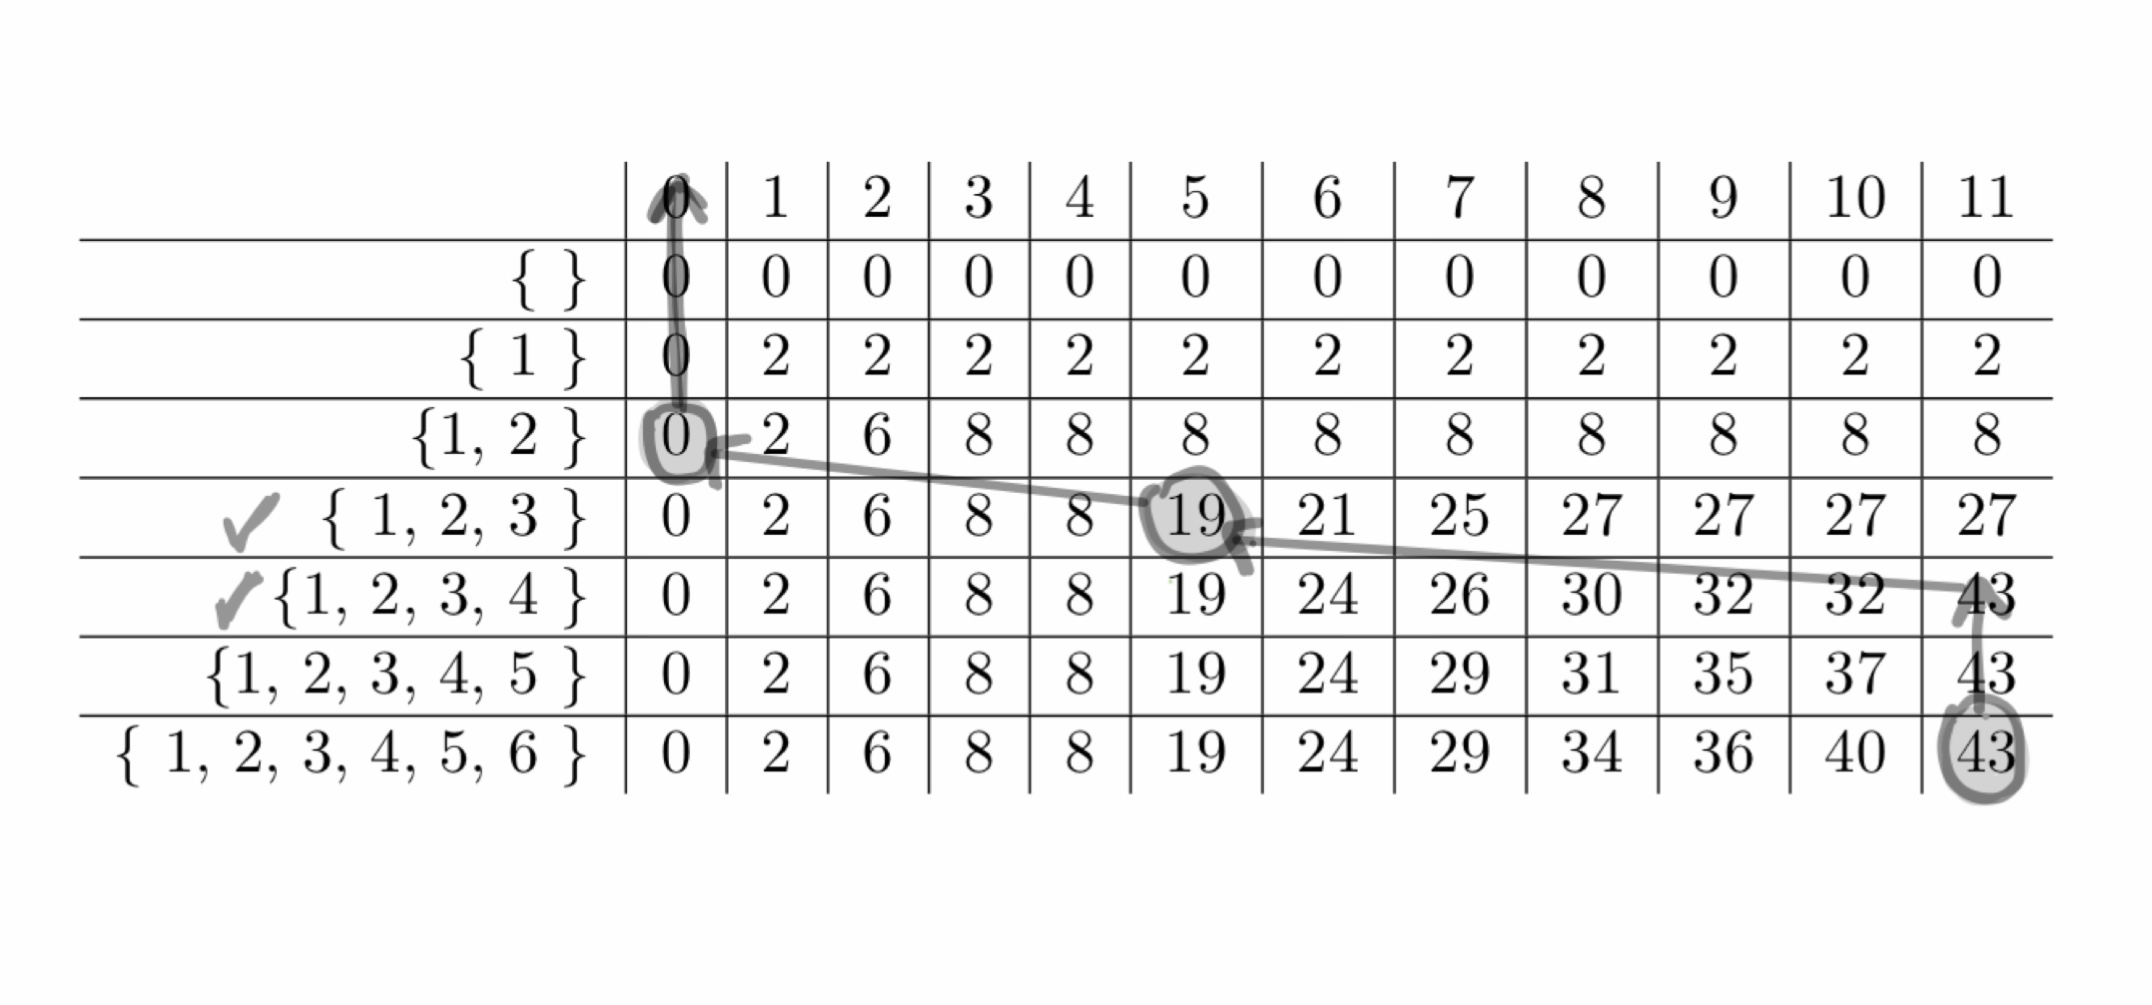
\includegraphics[width=0.8\textwidth]{hw8q1} \\

Since the table is filled in using this recurrence:\\
$If w<w_i: OPT(i,w)=OPT(i-1,w)$ \\
Otherwise: $OPT(i,w)=max(OPT(i-1,w), v_i+OPT(i-1,w-w_i)$ \\
Then the optimal subset of items is obtained through the following steps: 
\begin{enumerate}
\item Begin in the bottom right most cell of the table, at position OPT[i,w] which denotes the max profit. 
\item Trace up column w,  until you reach a row $r$ such that the value in the column directly above is different. That is when $OPT[r-1, w] \ne OPT[r,w]$. In this case, add the $r$th item to the subset. 
\item Now subtract the value of the $r$th item from the value in cell $OPT[r,w]$. 
\item Trace up and to the left until you find that corresponding value
\item Now repeat steps 2-5 until you reach OPT[0,0]. 
\end{enumerate}
Thus the optimal-value subset of items is $OPT = \{4,3\}$ \\


\end{proof}


\end{required}


\newpage
\begin{required}
Recall the sequence alignment problem where the cost of {\em sub} and the cost of {\em indel} are all $1$. Given the following table of optimal cost of aligning the strings EXPONEN and POLYNO, draw the backward path consisting of backward edges to find the minimal-cost set of edit operations that transforms EXPONEN to POLYNO. Besides indicating the backward path, you must also give the minimal-cost set of edit operations.  Clearly explain your work. 
 % ----- FIGURE -----
        \begin{figure}[h!]
        \begin{center}
        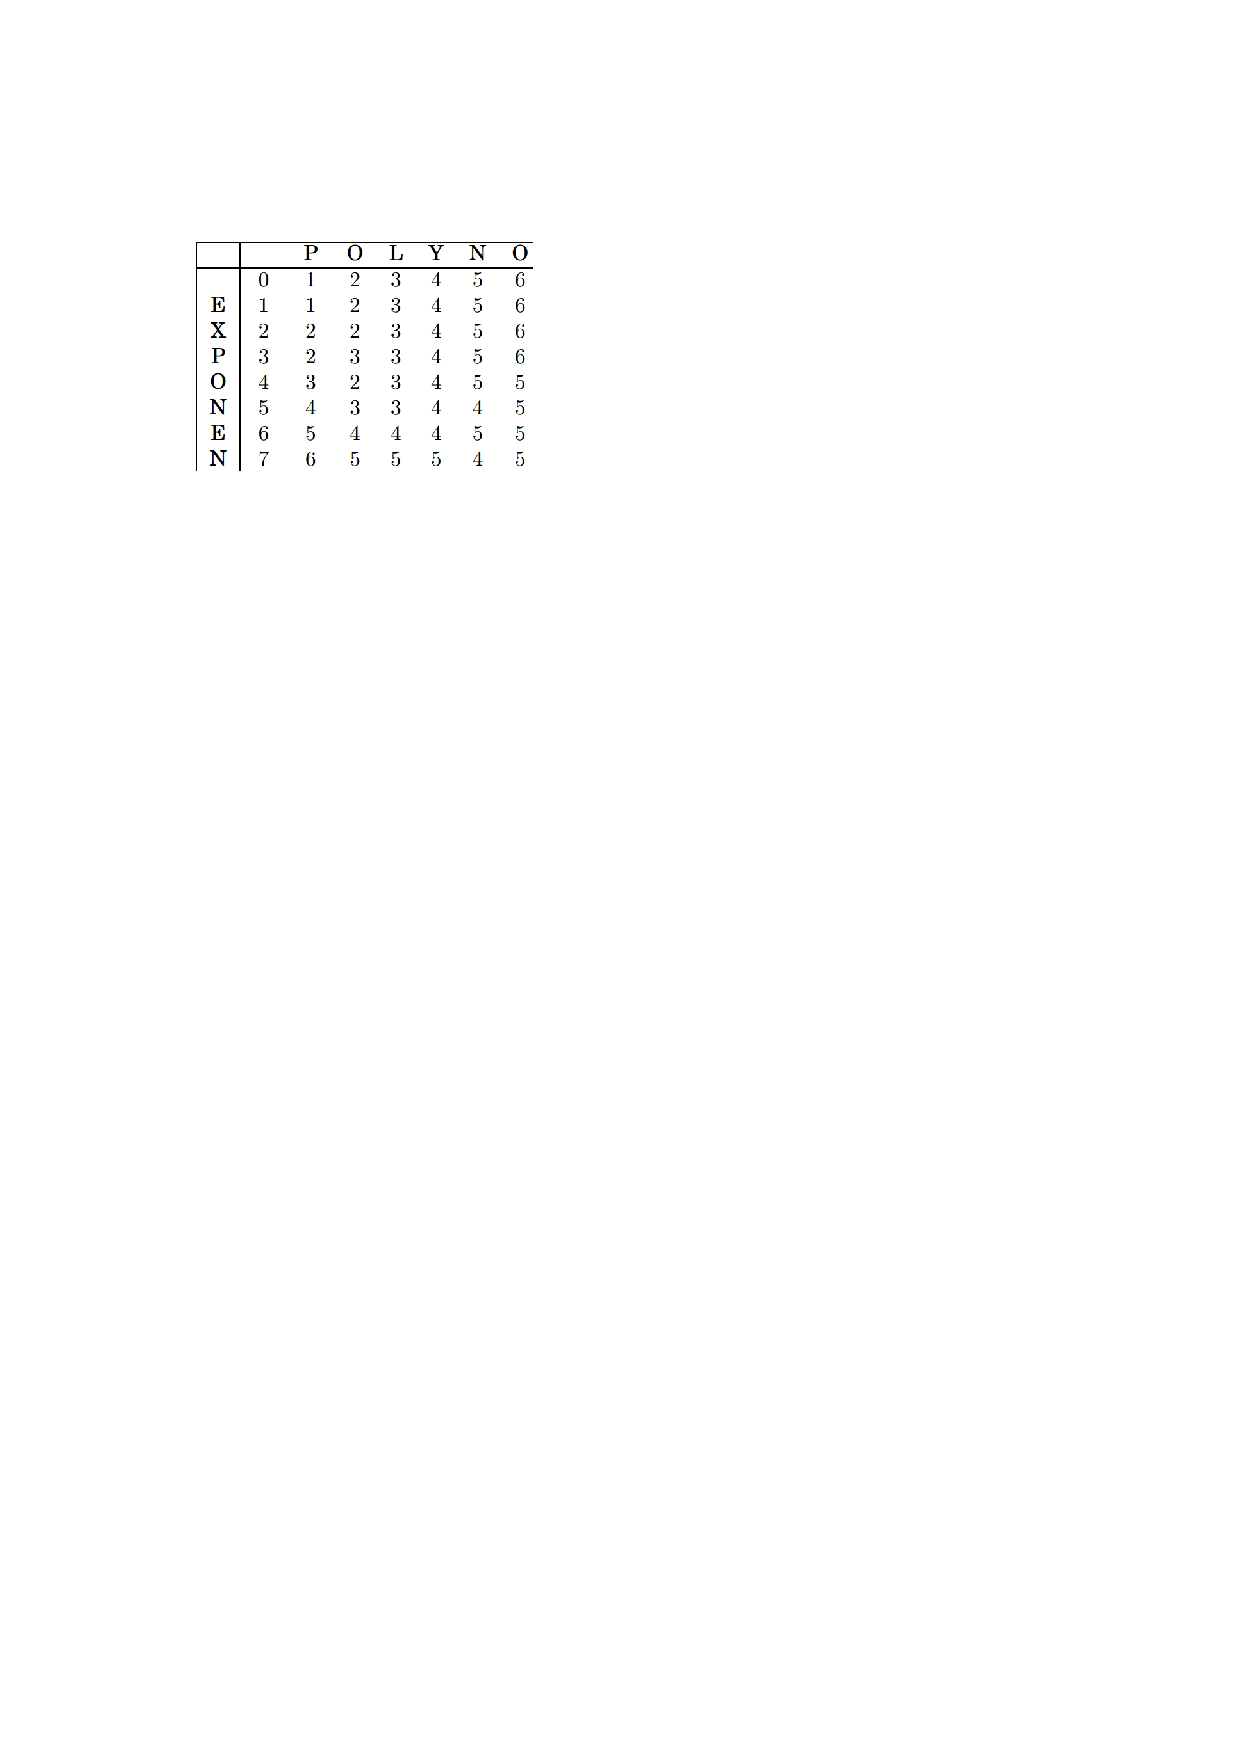
\includegraphics[scale=0.90]{exp_poly.pdf} 
        \end{center}
        \end{figure}
        % ----------

\begin{proof}[Answer]
%Your answer here
The backward path is seen below:  \\
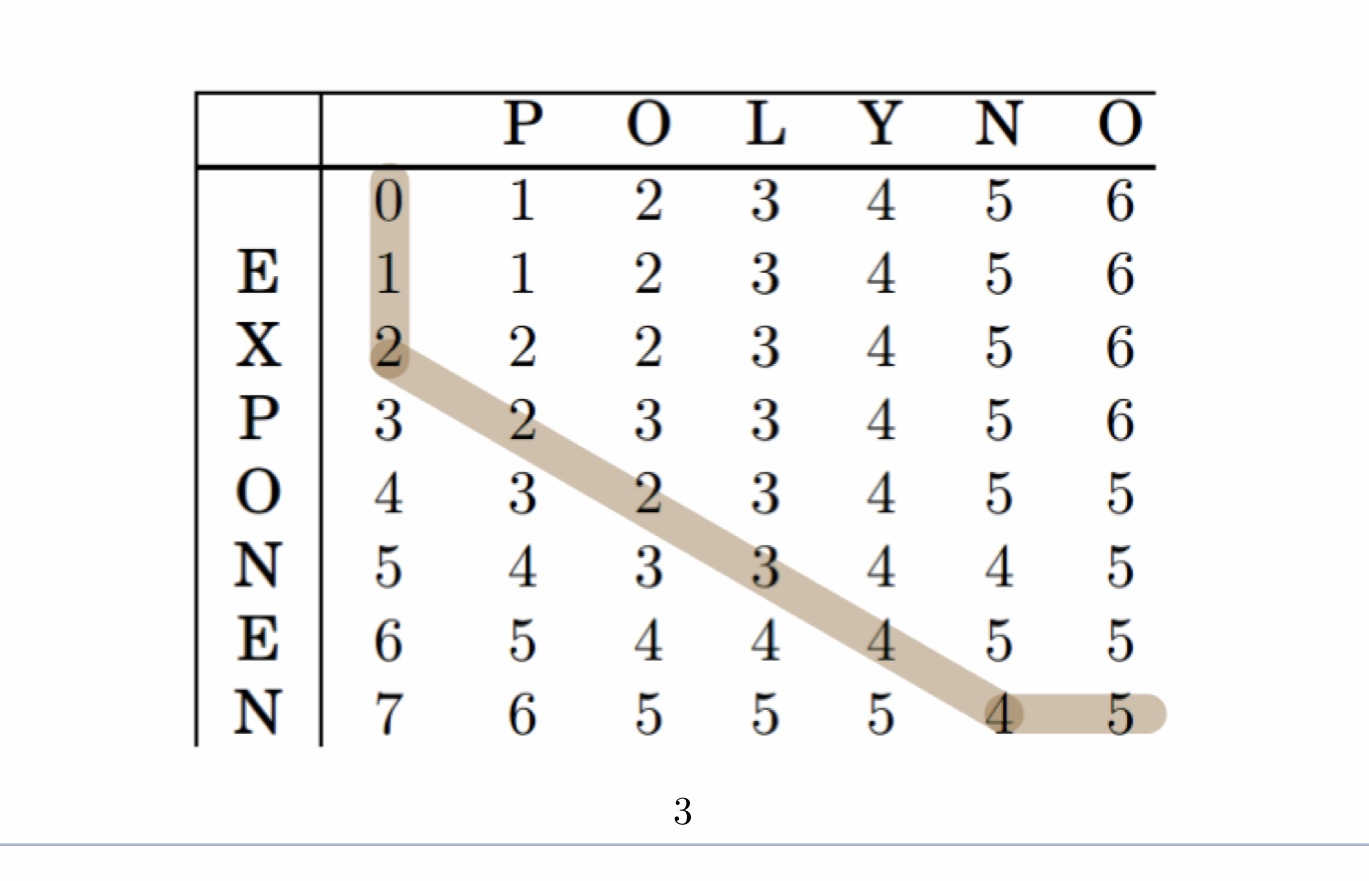
\includegraphics[width=0.5\textwidth]{hw8q2} \\

The minimal-cost set of edit operations is obtained through the following steps: 
To extract the minimum-cost alignments, we examine the sequences of choices made to arrive at $S(7,6)= 5$. Specifically, find the minimum cost path backwards through the DAG to S(0,0). Since We know the table was filled in based on the following recurrence relation, we can extract the minimal cost set of edit operations.\\
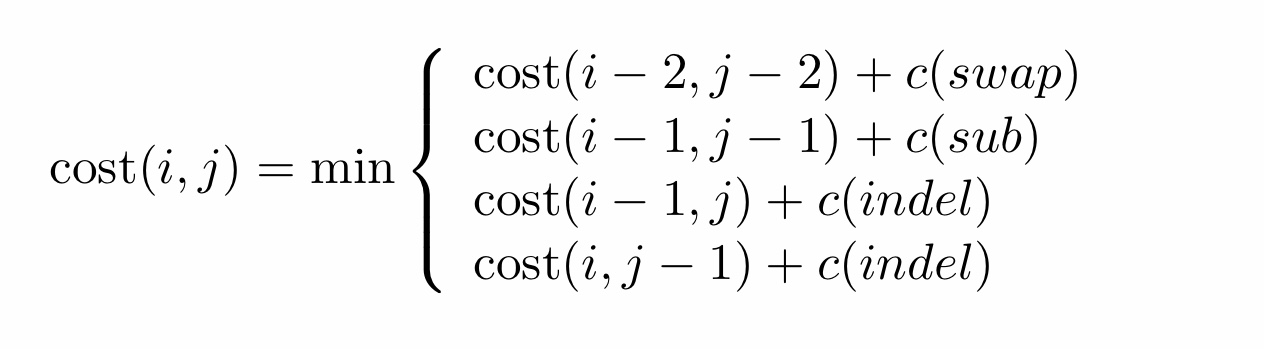
\includegraphics[width=0.5\textwidth]{hw8recur} \\
\begin{itemize}
\item A down move represents an $insertion$ operation, as it corresponds to the case when $cost(i,j)=cost(i-1,j)+1$ or $cost(i,j)=cost(i,j-1)+1$ 
\item A left move represents a $deletion$ operation, as it is when $cost(i,j)=cost(i-1,j)+1$ or $cost(i,j)=cost(i,j-1)+1$ 
\item A single diagonal move is a $substitution$, which is when $cost(i,j)=cost(i-1,j-1)+1$
\item Double diagonal moves are a $swap$ as it corresponds to $cost(i,j)=cost(i-2,j-2)+2$
\end{itemize}
The below figure shows this path and the corresponding alignment is 
\begin{align*}
&\text{- - POLYNO} \\
&\text{EXPONEN - }\\
&\text{ i   i }| \text{        } | \text{  s    s  }|\text{  d }
\end{align*}
for a total cost of 3 $indels$ and 2 $subs$, or 5 overall. 


\end{proof}

\end{required}

\newpage
\section{Standard 23- Dynamic Programming: Bellman-Ford Algorithm}

\begin{required}

Consider the weighted directed graph $G(V, E, w)$ pictured below. Work through the Bellman-Ford algorithm with the destination vertex $C$. 
\begin{itemize}
\item Clearly specify the cost $d(v)$ of the current  best path from each node $v\in V$ to $C$ as well as the corresponding successor node  at each iteration/pass. You may want to make a table to store the costs and successors.

\item Give the shortest path tree, i.e., the union of all the shortest paths to $C$ from all other vertices. For your convenience, you may want to modify the ``latex code" for the given graph to draw the shortest path tree.

\end{itemize}

\definecolor {processblue}{cmyk}{0.96,0,0,0}
\begin{center}
	\begin {tikzpicture}[-latex ,auto ,node distance =1.5cm and 2cm ,on grid ,
	semithick ,
	state/.style ={ circle ,top color =white , bottom color = processblue!20 ,
	draw,processblue , text=blue , minimum width =0.5 cm}, scale=0.5]

	\node[state] (A) {$A$};
	\node[state] (B) [above right = of A] {$B$};
	\node[state] (C) [below right = of A] {$C$};
	\node[state] (F) [below right = of B] {$F$};
	\node[state] (D) [above right = of F] {$D$};
	\node[state] (E) [below right = of F] {$E$};
	
	
	\path (A) edge node[above] {$6$} (B);
	\path (A) edge node[above] {$11$} (C);
	\path (B) edge node[above] {$1$} (F);
	\path (B) edge node[above] {$1$} (D);
	\path (F) edge node[above] {$1$} (A);
	\path (E) edge node[above] {$1$} (C);
	\path (D) edge node[above] {$3$} (F);	
	\path (F) edge node[above] {$5$} (E);
	\path (F) edge node[above] {$2$} (C);
	
	\end{tikzpicture}  
\end{center}




\begin{proof}[Answer]
%Your answer here

Apply Bellman-Ford to the graph: \\
Let $c(u,v)$ denote cost of the edge from vertex u to vertex v. Let $D(v)$ denote the cost of the current path from vertex v to the destination vertex C. 
\begin{enumerate}
\item 1st iteration: begin by examining source vertex C incoming edges. 
	\begin{itemize}
	\item Poll edge (A,C): $D(A)=\infty > D(C)+c(A,C)=0+11$ so set $D(A)=11$ and $successor[A]=C$
	\item Poll edge (F,C): $D(F)=\infty > D(C)+c(F,C)=0+2$ so set $D(F)=2$ and $successor[F]=C$
	\item Poll edge (E,C): $D(E)=\infty > D(C)+c(E,C)=0+1$ so set $D(E)=1$ and $successor[E]=C$
	\end{itemize}
\item 2nd iteration:examine the incoming edges for each of the updated vertices, which were A, F, C 
	\begin{itemize}
	\item Poll edge (F,A): $D(F)=2 < D(A)+c(F,A)=11+1=12$ so no change
	\item Poll edge (F,E): $D(F)=2 < D(E)+c(F,E)=5+1$ so no change
	\item Poll edge (D,F): $D(D)=\infty > D(F)+c(F,F)=2+3$ so set $D(D)=5$ and $successor[D]=F$
	\item Poll edge (B,F): $D(B)=\infty > D(F)+c(E,C)=2+1$ so set $D(B)=3$ and $successor[B]=F$
	\end{itemize}
\item 3rd iteration:examine the incoming edges for each of the updated vertices, which were D,B 
	\begin{itemize}
	\item Poll edge (A,B): $D(A)=11> D(B)+c(A,B)=3+6=9$ so set $D(A)=9$ and $successor[A]=B$
	\item Poll edge (B,D): $D(B)=3 < D(D)+c(B,D)=5+1=6$ so no change
	\end{itemize}
\item 4th iteration:examine the incoming edges for each of the updated vertices, which was A
	\begin{itemize}
	\item Poll edge (F,A): $D(F)=2 < D(A)+c(F,A)=11+1=12$ so no change
	\end{itemize}
\item 5th iteration:no updates made
\end{enumerate}
At the end of the algorithm the paths are the following\\
\begin{itemize}
\item A-B-F-C with cost of 9
\item B-F-C with cost 3
\item F-C with cost 2
\item E-C with cost 1
\item D-F-C with cost 5
\end{itemize}
See the shortest path tree below \\
\definecolor {processblue}{cmyk}{0.96,0,0,0}
\begin{center}
	\begin {tikzpicture}[-latex ,auto ,node distance =1.5cm and 2cm ,on grid ,
	semithick ,
	state/.style ={ circle ,top color =white , bottom color = processblue!20 ,
	draw,processblue , text=blue , minimum width =0.5 cm}, scale=0.5]

	\node[state] (A) {$A$};
	\node[state] (B) [above right = of A] {$B$};
	\node[state] (C) [below right = of A] {$C$};
	\node[state] (F) [below right = of B] {$F$};
	\node[state] (D) [above right = of F] {$D$};
	\node[state] (E) [below right = of F] {$E$};
	
	
	\path (A) edge[color= red] node[above] {$6$} (B);
	\path (A) edge node[above] {$11$} (C);
	\path (B) edge[color= red] node[above] {$1$} (F);
	\path (B) edge node[above] {$1$} (D);
	\path (F) edge node[above] {$1$} (A);
	\path (E) edge[color= red] node[above] {$1$} (C);
	\path (D) edge[color= red] node[above] {$3$} (F);	
	\path (F) edge node[above] {$5$} (E);
	\path (F) edge[color= red] node[above] {$2$} (C);
	
	\end{tikzpicture}  
\end{center}


\begin{table}[htp]
\centering
\caption{Initialization}
\begin{tabular}{|l|l|l|} 
\hline
\rowcolor[rgb]{0.753,0.753,0.753} Node & Cost     & Successor  \\ 
\hline
A                                      & $\infty$ & null       \\ 
\hline
B                                      & $\infty$ & null       \\ 
\hline
C                                      & 0        & C          \\ 
\hline
D                                      & $\infty$ & null       \\ 
\hline
E                                      & $\infty$ & null       \\ 
\hline
F                                      & $\infty$ & null       \\
\hline
\end{tabular}
\end{table}
\begin{table}[htp]
\centering
\caption{1st Iteration}
\begin{tabular}{|l|l|l|} 
\hline
\rowcolor[rgb]{0.753,0.753,0.753} Node & Cost                & Successor           \\ 
\hline
\textcolor{red}{A}                     & \textcolor{red}{11} & \textcolor{red}{C}  \\ 
\hline
B                                      & $\infty$            & null                \\ 
\hline
C                                      & 0                   & C                   \\ 
\hline
D                                      & $\infty$            & null                \\ 
\hline
\textcolor{red}{E}                     & \textcolor{red}{1}  & \textcolor{red}{C}  \\ 
\hline
\textcolor{red}{F}                     & \textcolor{red}{2}  & \textcolor{red}{C}  \\
\hline
\end{tabular}
\end{table}
\begin{table}[htp]
\centering
\caption{2nd Iteration}
\begin{tabular}{|l|l|l|} 
\hline
\rowcolor[rgb]{0.753,0.753,0.753} Node & Cost               & Successor           \\ 
\hline
A                                      & 11                 & C                   \\ 
\hline
\textcolor{red}{B}                     & \textcolor{red}{3} & \textcolor{red}{F}  \\ 
\hline
C                                      & 0                  & C                   \\ 
\hline
\textcolor{red}{D}                     & \textcolor{red}{5} & \textcolor{red}{F}  \\ 
\hline
E                                      & 1                  & C                   \\ 
\hline
F                                      & 2                  & C                   \\
\hline
\end{tabular}
\end{table}
\begin{table}[htp]
\centering
\caption{3rd Iteration}
\begin{tabular}{|l|l|l|} 
\hline
\rowcolor[rgb]{0.753,0.753,0.753} Node & Cost               & Successor           \\ 
\hline
\textcolor{red}{A}                     & \textcolor{red}{9} & \textcolor{red}{B}  \\ 
\hline
B                                      & 3                  & F                   \\ 
\hline
C                                      & 0                  & C                   \\ 
\hline
D                                      & 5                  & F                   \\ 
\hline
E                                      & 1                  & C                   \\ 
\hline
F                                      & 2                  & C                   \\
\hline
\end{tabular}\end{table}
\begin{table}[htp]
\centering
\caption{4th Iteration}
\begin{tabular}{|l|l|l|} 
\hline
\rowcolor[rgb]{0.753,0.753,0.753} Node & Cost & Successor  \\ 
\hline
A                                      & 9    & B          \\ 
\hline
B                                      & 3    & F          \\ 
\hline
C                                      & 0    & C          \\ 
\hline
D                                      & 5    & F          \\ 
\hline
E                                      & 1    & C          \\ 
\hline
F                                      & 2    & C          \\
\hline
\end{tabular}
\end{table}
\begin{table}
\centering
\caption{5th Iteration}
\begin{tabular}{|l|l|l|} 
\hline
\rowcolor[rgb]{0.753,0.753,0.753} Node & Cost & Successor  \\ 
\hline
A                                      & 9    & B          \\ 
\hline
B                                      & 3    & F          \\ 
\hline
C                                      & 0    & C          \\ 
\hline
D                                      & 5    & F          \\ 
\hline
E                                      & 1    & C          \\ 
\hline
F                                      & 2    & C          \\
\hline
\end{tabular}
\end{table}

\end{proof}


\end{required}

\end{document} % NOTHING AFTER THIS LINE IS PART OF THE DOCUMENT
